\subsection{Smart contracts}

As noted before, the smart contracts are small programs that run on the Ethereum Virtual Machine. They can be deployed by anyone, who has access to the Ethereum network and has enough funds to cover the necessary gas for the contract deployment. Smart contracts only exist within the realm of the Ethereum blockchain~\cite{JohnWeldon2016BuildingContract} and they can only be accessed by the nodes participating in the network. We could use the blockchain explorers to find out about existing smart contracts and we would be able see the compiled bytecode. However, this would not give us many answers about the purpose of the smart contract, since the bytecode is not easily comprehensible. To better investigate, how various smart contracts are used, we decided to browse a DApp repository instead.

To investigate Smart contracts for this section, we decided to browse a curated repository of decentralised applications \textit{State of the DApps}\footnotemark.%
% 
\footnotetext{\url{https://www.stateofthedapps.com/}, accessed 23-05-2018}
% 
State of the DApps is currently the only service offering similar listings. This repository is submission based (it does not search for new DApps on the blockchain, rather it accepts submissions from developers that wish to have their DApp enlisted), thus is not exhaustive. Anyone can submit a DApp and it will be added to the repository, unless it is offensive or inappropriate, in which case it will be removed. According to the repository, the decentralised applications span many fields, ``\textit{covering different fields such as health, Ponzi schemes, games, virtual reality, artificial intelligence, education, registries, job markets, [...] and many more}''\footnotemark. 
% 
\footnotetext{\url{https://www.stateofthedapps.com/about}, accessed 18-05-2018}

Currently, the repository contains more than 1000 DApps. We searched for the keywords `exchange' and `currency', and tried to find a similar product to our envisioned system, but we could not find any DApps that would allow exchange of fiat currencies. The closest match to an exchange platform is arguably the \textit{IDEX} trading platform\footnotemark which allows trading of ERC20 tokens on the Ethereum network. Tokens are a specific use case of the smart contracts that can represent different assets, such as vouchers, documents, shares or even objects in the real world~\cite{NathanReiff2017WhatEthereum}. They can also be used as \textit{subcurrencies}, existing only on the Ethereum network. ERC20 is a standardisation effort to maintain a common set of methods among these tokens.%
% 
\footnotetext{\url{https://idex.market/eth/aura}, accessed 22-05-2018}
%
IDEX is a decentralised application that allows trading these standardised ERC20 tokens. The trading logic is executed by a smart contract, which can be viewed and verified using a blockchain explorer\footnotemark.
% 
\footnotetext{\url{https://etherscan.io/address/0x2a0c0dbecc7e4d658f48e01e3fa353f44050c208}, accessed 22-05-2018}

Since ERC20 tokens exist within the Ethereum blockchain, the IDEX does not need to retrieve any data from any external sources. However it shows us, that a decentralised trading application indeed can operate its business logic on a public and verifiable smart contract. The main contract of the IDEX exchange has more than 2 million transactions and current balance of more than 43 000 ETH, which clearly shows users' interest in the platform. Figure \ref{fig:idex} depicts the front page of the IDEX platform.

\begin{figure}[ht]
    \centering
    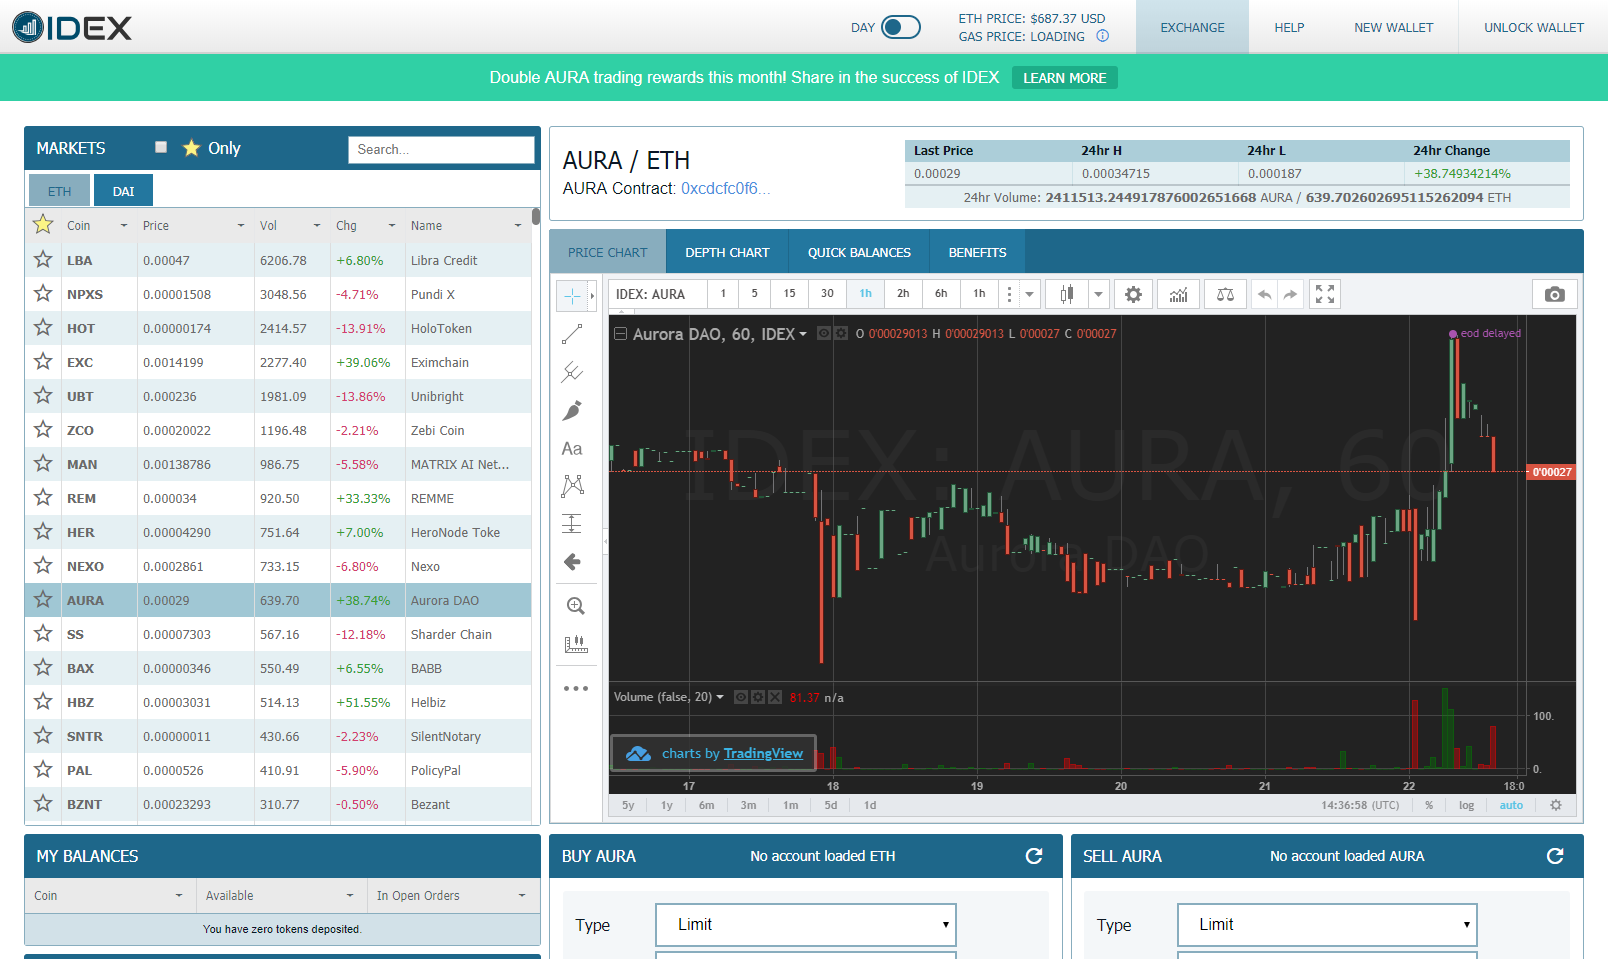
\includegraphics[width=\textwidth]{idex}
    \caption{Front page of the IDEX trading platform.}
    \label{fig:idex}
\end{figure}

There are also numerous escrow services in the State of the DApps repository, but mostly they only provide their services for Ether to Ether or token to token transactions. We also searched the repository for any DApps that would interact with the real-world data. The most notable example is a flight-cancellation insurance provider Etherisc\footnotemark. It provides an insurance on flight delays and cancellations, promising an automated payout, if the flight gets cancelled or delayed. On their website however, the possibility to book an insurance with Ether is currently disabled and the smart contract featured by Etherisc in the State of the DApss repository is on a Ropsten test network only. We could not locate any contract associated with Etherisc on the mainnet, so the actual usage of this application could not be determined.
% If it does work however, it needs to learn flight status data for its execution.
% 
\footnotetext{\url{https://fdd.etherisc.com/}, accessed 22-05-2018}
